\documentclass[a4paper]{article}
\usepackage[utf8]{inputenc}
\usepackage{polski}
\usepackage[polish]{babel}
\usepackage[T1]{fontenc}
\usepackage{graphicx}
\usepackage{verbatim}
\usepackage{float}
\usepackage{minted}
\usepackage{microtype}
\usepackage{shortvrb}
\usepackage{amsmath}

\let\olditemize=\itemize \let\endolditemize=\enditemize \renewenvironment{itemize}{\olditemize \itemsep0em}{\endolditemize}

\title{TEMAT ĆWICZENIA: OpenGL – interakcja z użytkownikiem}
\author{Marcel Guzik}

\begin{document}
\section{Wprowadzenie}

Ćwiczenie ma za zadanie pokazać, jak przy pomocy funkcji biblioteki OpenGL z
biblioteką GLUT można zrealizować prostą interakcję, polegające na sterowaniu
ruchem obiektu i położeniem obserwatora w przestrzeni 3D. Do sterowania służyla
będzie mysz. Ponadto zostaną zilustrowanie sposoby prezentacji obiektów
trójwymiarowych w rzucie perspektywicznym.


Finalny program realizuje:
\begin{itemize}
    \item Po uruchomieniu programu, w położeniu początkowym rysowane jest jajko
    \item Przy wciśniętym lewym klawiszu myszy, ruch kursora myszy w kierunku
          poziomym powinien powodować proporcjonalną zmianę azymutu kąta
          $\Theta$.
    \item Przy wciśniętym lewym klawiszu myszy, ruch kursora myszy w kierunku
          pionowym powinien powodować proporcjonalną zmianę kąta elewacji
          $\Phi$.
    \item Przy wciśniętym prawym klawiszu myszy, ruchy kursora myszy w kierunku
          pionowym winien realizować zmianę promienia R.
    \item Możliwa jest zmiana rysowanego modelu pomiędzy różnymi modelami jaja
          oraz czajnikiem.
\end{itemize}

\begin{figure}[H]
    \centering
    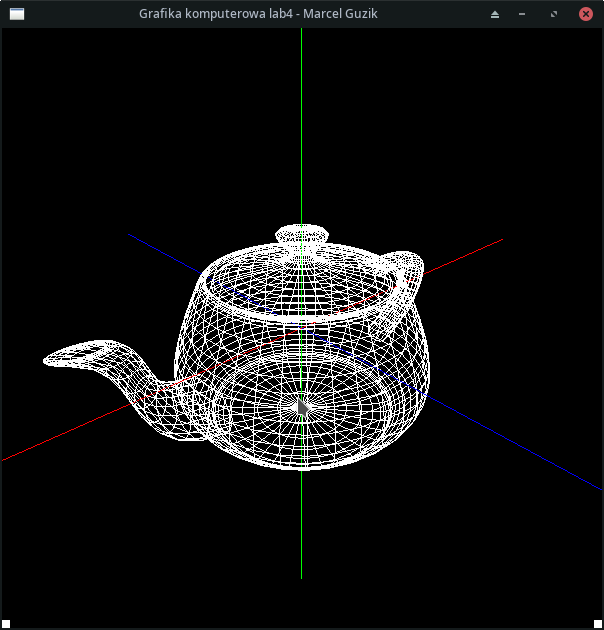
\includegraphics[width=0.48\textwidth]{teapot}
    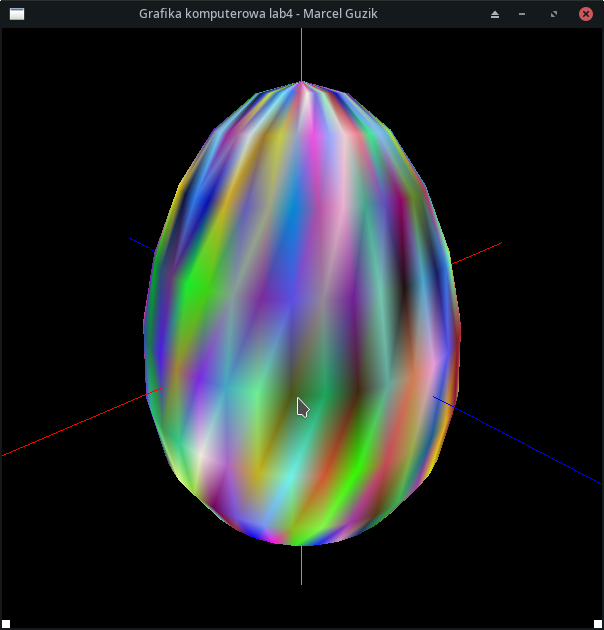
\includegraphics[width=0.48\textwidth]{egg}
    \caption{Widok czajnika oraz jaja}
\end{figure}

\textit{Uwaga: pojęcia ``obserwator'' oraz ``kamera'' są używane wymiennie.}

\section{Teoria}
\subsection{Stos transformacji macierzowych}

Aby wyświetlić przestrzeń trójwymiarową na dwuwymiarowym ekranie komputera,
niezbędne jest wykonanie przekształceń systemów współrzędnych, które
przetransformują współrzędne rysowanych obiektów na znormalizowane współrzędne
urządzenia (NDC). Możemy wykonywać te przekształcenia krokowo, za pomocą
mnożenia przez siebie kolejnych macierzy. Diagram przekształceń widoczny jest na
rysunku \ref{fig:coordinates}.

\begin{figure}[H]
    \centering
    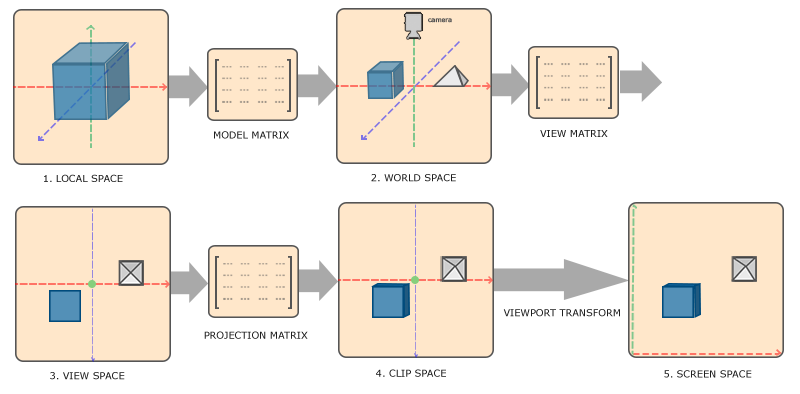
\includegraphics[width=\textwidth]{coordinate_systems}
    \caption{Kolejne kroki przekształceń systemu współrzędnych za pomocą transformacji macierzowych}
    \label{fig:coordinates}
\end{figure}

\begin{enumerate}
    \item Współrzędne lokalne to współrzędne obiektu relatywne dla niego samego.
          Np. dla naszego jajka początek układu lokalnych współrzędnych znajduje
          się u jego podstawy. Musimy zatem wykonać translację za pomocą
          macierzy modelu by wycentrować jajko w naszym układzie współrzędnych.
    \item Następnym krokiem jest transformacja współrzędnych lokalnych do
          współrzędnych przestrzeni świata, gdzie współrzędne opisują pozycję
          obiektów w świecie. Są one relatywne do arbitralnie wybranego początku
          układu współrzędnych.
    \item Następnie przekształcamy współrzędne przestrzeni świata do
          współrzędnych przestrzeni widoku za pomocą macierzy widoku. Jest to
          przestrzeń, w której początkiem układu współrzędnych jest pozycja
          obserwatora i kierunek w którym jest on zwrócony. W tym miejscu nie
          jest jeszcze zdefiniowany zakres widoczności obserwatora, więc żadne
          wierzchołki nie są usuwane.
    \item Przestrzeń widoku chcemy następnie przyciąć tak, by tylko obiekty
          widziane przez obserwatora znajdowały się w zdefiniowanej przestrzeni
          oraz by ograniczyć zakres współrzędnych do $(-1.0, 1.0)$, czyli tak by
          wyrazić tą przestrzeń w znormalizowanych współrzędnych urządzenia
          (Normalized Device Coordinates) możliwych do wyświetlenia przez
          OpenGL.
    \item Jako ostatni krok, przekształcamy ``przycięte'' współrzędne do
          współrzędnych ekranu (czyli upraszczając, po prostu w piksele).

\end{enumerate}

Na rysunku widoczne są 3 różne macierze, jednak w trybie Fixed Function Pipeline
w OpenGL mamy dostęp do tylko 2 macierzy: \verb|GL_MODELVIEW| oraz
\verb|GL_PROJECTION|. Jak wskazuje nazwa, macierze modelu oraz widoku są ze
sobą połączone.

Transformacje z przestrzeni ``uciętej'' do przestrzeni ekranu przez funkcję
\texttt{glViewport()} były opisywane w sprawozdaniu do ćwiczenia nr 2,
dlatego nie będą opisywane w niniejszym sprawozdaniu.

Aby zaimplementować ruszającą się kamerę, niezbędne będzie wykonanie macierzy
widoku, tudzież macierzy \verb|GL_MODELVIEW| oraz macierzy rzutowania. Macierz
modelu i widoku ustawia funkcja \texttt{gluLookAt()}, natomiast macierz
rzutowania ustawia funkcja \texttt{gluPerspective()}.

\subsection{Pozycja kamery i macierz widoku}

Do zdefiniowania pozycji kamery potrzebujemy czterech wektorów:

\begin{itemize}
    \item Wektor pozycji kamery w systemie współrzędnych świata: $p$
    \item Wersor definiujący kierunek w który skierowana jest kamera: $\hat{z}$
    \item Wersor osi x: $\hat{x}$
    \item Wersor osi y: $\hat{y}$
\end{itemize}

\begin{figure}[H]
    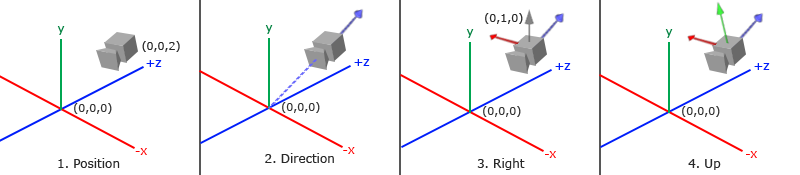
\includegraphics[width=\textwidth]{camera_axes}
    \caption{Proces uzyskiwania wektorów położenia oraz wersorów $\hat{x}$,
        $\hat{y}$, $\hat{z}$ kamery}
\end{figure}

Zadaniem macierzy widoku jest przetransformowanie systemu współrzędnych w taki
sposób, by nowy system opisywał położenie obiektów tak, jak są one widoczne z
punktu widzenia obserwatora. W tym celu należy zastosować kombinację translacji,
skalowania oraz rotacji, które mają spełnić następujące warunki:

\begin{itemize}
    \item Obserwator znajduje się w początku nowego układu współrzędnych.
    \item Obserwator skierowany jest w stronę danego punktu (inaczej mówiąc:
          oś $z$ przebiega przez dany punkt oraz obserwatora)
    \item System współrzędnych obracany jest zgodnie z wartościami nowych
          wektorów $x$ oraz $y$ ustalonych przez obserwatora.
\end{itemize}

Efektem jest następująca macierz która realizuje transformację do systemu
współrzędnych widoku:

\begin{figure}[H]
    \[
        \begin{bmatrix}
            \hat{x}_x & \hat{x}_y & \hat{x}_z & 0 \\
            \hat{y}_x & \hat{y}_y & \hat{y}_z & 0 \\
            \hat{z}_x & \hat{z}_y & \hat{z}_z & 0 \\
            0         & 0         & 0         & 1
        \end{bmatrix}
        \cdot
        \begin{bmatrix}
            1 & 0 & 0 & -P_x \\
            0 & 1 & 0 & -P_y \\
            0 & 0 & 1 & -P_z \\
            0 & 0 & 0 & 1
        \end{bmatrix}
    \]
    \caption{Macierz widoku}
\end{figure}

Gdzie lewa macierz jest odpowiedzialna za rotację, a prawa za translację.

\subsection{Rzutowanie perspektywistyczne}
W poprzednim ćwiczeniu stosowano rzutowanie równoległe, a dokładniej jego
szczególny przypadek zwany rzutem ortograficznym. Do realizacji rzutowania
ortograficznego służy funkcja \verb|glOrtho()|. W rzucie ortograficznym rzutnia,
czyli płaszczyzna na której powstawał obraz, była równoległa do płaszczyzny
tworzonej przez osie x i y, a proste rzutowania biegły równoległe do osi z.

Ze względu na to, że proste rzutowania są równoległe do osi z, przesuwanie
obiektu wzdłuż tej osi nie spowoduje żadnego efektu na obrazie. Aby umożliwić
pokazanie efektów przemieszczeń obiektu we wszystkich osiach nalely zastosować
rzutowanie perspektywiczne. Rzut perspektywiczny jest lepszy od równoległego nie
tylko ze względu na możliwość prezentacji przemieszczeń, pozwala także lepiej
pokazać na płaszczyźnie geometrii trójwymiarowego obiektu.

Poniżej znajduje się rysunek bryły widoczności zdefiniowanej przez funkcję
\verb|gluPerspective()|. Bryły znajdujące się w całości poza bryłą widoczności
kamery nie są rysowane.

\begin{figure}[H]
    \centering
    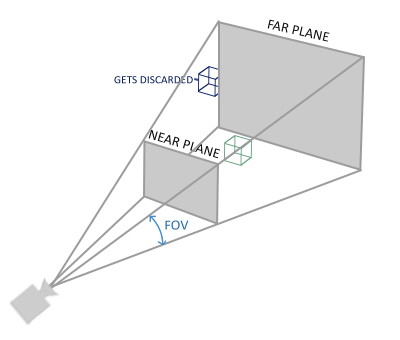
\includegraphics[width=0.5\textwidth]{perspective_frustum}
    \caption{Bryła widoczności zdefiniowana przez macierz rzutu perspektywistycznego}
\end{figure}

\subsection{Rotacja}

Efektywnie, rotacja realizowana przez program składa się z dwóch elementów:

\begin{enumerate}
    \item \textbf{Zakrzywienie ruchu obserwatora.} Obserwator pozostaje w
          zdefiniowanej odległości $R$ od środka układu współrzędnych. Poprzez
          ruch myszą w dwóch dostępnych osiach, obserwator porusza się ruchem
          kątowym za pomocą dwóch kątów, azymutu $\Theta$, oraz elewacji $\Phi$.

          System równań określający możliwe pozycje obserwatora wygląda
          następująco:

          \begin{figure}[H]
              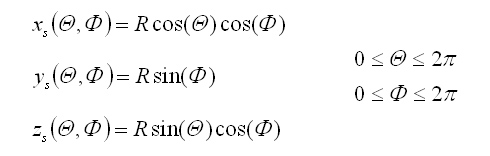
\includegraphics[width=\textwidth]{rotation-equations}
              \caption{System równań określający pozycję obserwatora}
          \end{figure}

    \item \textbf{Obrót obserwatora w kierunku początku układu współrzędnych.}
          Ta część zrealizowana jest w funkcji \verb|gluLookAt()| i jest częścią
          macierzy widoku. Przekształca ona system współrzędnych, możliwie
          obracając go tak, by osie $x$ oraz $y$ odpowiadały osiom $x$ oraz $y$
          powierzchni ekranu, oraz by oś $z$ układała się ``wgłąb'' ekranu.
\end{enumerate}

\section{Wykonanie programu}

Przekształcenie przestrzeni świata w przestrzeń widoku wykonuje funkcja
\texttt{gluLookAt()}. Przyjmuje ona jako argumenty:

\begin{itemize}
    \item wektor określający pozycję obserwatora
    \item punkt w kierunku którego zwrócony jest obserwator
    \item wektor określający kierunek górny z punktu widzenia obserwatora
\end{itemize}

Zakładając wywołanie \texttt{gluLookAt(p2, t, u)}, gdzie \verb|p2| to pozycja
obserwatora, \verb|t| to obiekt w stronę którego zwrócony jest obserwator, a
\verb|u| to wektor definiujący kierunek górny we współrzędnych świata, funkcja
uzyskuje argumenty w sposób następujący:

\[p = p2\]
\[\hat{z} = \frac{p - t}{|p-t|}\]
\[\hat{x} = \frac{u \times \hat{z}}{|u \times \hat{z}|}\]
\[\hat{y} = \hat{z} \times \hat{x}\]

Przekształcenie przestrzeni widoku w przestrzeń ``uciętą'' wykonuje funkcja
\texttt{gluPerspective()}. Jest ona zdefiniowana następująco:

\mint{C}{void gluPerspective(double fovy, double aspect, double zNear, double zFar)}

Kolejne argumenty to:

\begin{itemize}
    \item Pole widzenia w osi $y$
    \item Proporcje osi $x$ do osi $y$
    \item Minimalna odległość rysowania w osi $z$
    \item Maksymalna odgległość rysowania w osi $z$
\end{itemize}

Ponadto, dalsze wytłumaczenie nowego kodu jest dostępne w postaci komentarzy.
Nowy kod źródłowy:

\inputminted{C}{funcs.c}

\section{Problemy}

\subsection{Zmiana orientacji kamery przy przekroczeniu osi $y$}

Przez wykorzystanie funkcji \verb|gluLookAt()|, gdy rotacja przekraczała oś $y$,
następowała zmiana orientacji kamery tak, by górna krawędź widoku kamery była
skierowana w kierunku rosnących $y$, tzn. tak by kamera nie była ``do góry
nogami''. Skutkowało to skokową zmianą orientacji kamery oraz obrotu pokazywanego
obiektu.

Możliwe były następujące sposoby rozwiązania tego problemu:

\begin{itemize}
    \item Zablokować kąty rotacji tak by niemożliwe było przekroczenie osi $y$
    \item Gdy współrzędne kamery przekroczyły oś $y$, zmienić zwrot wektora
          $up$, tak by kamera pozostała ``do góry nogami''.
\end{itemize}

Do rozwiązania problemu zdecydowano się zablokowanie kątów rotacji.

\subsection{Niska rozdzielczość ruchów myszą}

Ponieważ funkcja obsługująca zdarzenia ruchu myszą otrzymuje od systemu
operacyjnego liczbę pikseli o którą poruszył się wskaźnik myszy, obracanie
widokiem może się niekiedy wydawać skokowe, szczególnie kiedy czułość myszy jest
niska i uruchamiamy program na ekranie o niskiej rozdzielczości.

Rozwiązaniem tego problemu byłoby pobieranie informacji o ruchu myszy nie
poprzez liczbę pikseli o którą poruszył się kursor, lecz jako bardziej
``surowe'' dane, określające poruszenie myszą bez względu na to czy kursor myszy
poruszył się na ekranie. Byłaby to liczba zmiennoprzecinkowa, która mogłaby być
arbitralnie mała dla bardzo niewielkich poruszeń myszą.

\end{document}